I dette kapitel vil den valgte platform, \legoms, kort blive beskrevet, sammen med en begrundelse for dette valg.
Yderligere argumenteres der for valg af API til NXTen.

\section{\legoms}\label{lego:mindstorms-nxt}
\legoms er et byggesæt, hvor det er muligt at bygge programmerbare robotter i \lego-klodser.

Til at bygge disse robotter, er der i \legoms nogle sensorer og aktuatorer. Sensorerne gør det muligt for robotten at modtage input fra sine omgivelser.
Ved brug af aktuatorerne kan robotten agere i verden og evt. reagere på inputs fra sine sensorer.

Ud over de originale \lego dele, er der også tredjeparts producenter, som har et udbud af andre typer sensorer og aktuatorer, der kan samarbejde med \legoms.

\subsection{NXT}
Denne sektion er baseret på \cite{nxt}, hvilket omhandler NXT 2.0, som er den version der bruges i dette projekt.
NXT Intelligent Brick (oftest kaldt blot 'NXT' eller 'brick') er hjernen i \legoms robotten.
Det er den der står for at modtage og behandle input fra sensorer, samt styre de monterede aktuatorer.
Et billede af NXT 2.0 kan ses på \cref{platform:nxt}.

\begin{figure}
\begin{center}
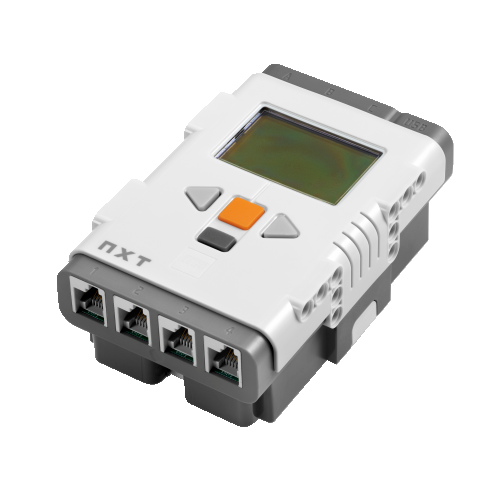
\includegraphics[scale=.5]{./graphics/nxt/brick}
\end{center}
\caption{NXT Intelligent Brick.}
\label{platform:nxt}
\end{figure}

\subsubsection{Porte}
NXTen har 3 motorporte (kaldet A, B og C) og 4 sensorporte (kaldet 1, 2, 3 og 4).

\subsubsection{Tilslutningsmuligheder}
Der kan kommunikeres med NXTen ved at tilslutte den til en anden enhed med USB-kabel eller Bluetooth.

\subsubsection{Feedback}
Til output har NXTen en 100 x 64 pixel LCD display, samt en 8 kHz højttaler.

\subsubsection{Styring}
NXTen kan styres på to måder:
Man kan sende kommandoer og modtage beskeder (for eksempel sensor aflæsninger) på en ekstern enhed (oftest en computer eller en anden NXT).
Alternativt kan programmer sendes (via Bluetooth eller USB) til NXTen, hvorfra de kan køres direkte, uafhængig af eksterne enheder.


\subsubsection{Tekniske specifikationer}
De tekniske specifikationer for NXT 2.0 kan ses i \cref{mindstorms:tekniske_spec} \cite{nxt}. 


\begin{table}[h]
\begin{tabular}{|c |c|}
\hline
Microcontroller & \shortstack{\\32-bit ARM7 microcontroller\\ 8-bit AVR controller}\\
\hline
RAM & \shortstack{ \\256 Kb FLASH, 64 Kb RAM \\ 4 Kb FLASH, 512 b RAM} \\
\hline
Kommuniation & \shortstack{ \\Bluetooth (Bluetooth Class II V2.0 compliant) \\ USB full speed port (12 Mbit/s)}\\
\hline
Input porte & 4 \\
\hline
Output porte & 3 \\
\hline
Display & 100 x 64 pixel LCD \\
\hline
Højttaler & 8 kHz lyd. 8-bit lydkanal og 2-16 kHz sample rate\\
\hline
Strømkilde & 6 AA batteries\\
\hline
\end{tabular}
\caption{\legoms NXT tekniske specifikationer.}
\label{mindstorms:tekniske_spec}
\end{table}


\subsection{Valg af \legoms}
Der er mange gode grunde til at vælge \legoms.
Her er givet fire overordnede punkter, der efterfølgende vil blive gennemgået:

\begin{itemize}
\item{Tilgængelighed}
\item{Nemt at gå til}
\item{Stort udvalg af sensorer}
\item{Mange muligheder ift. styring}
\end{itemize}

\subsubsection{Tilgængelighed}
Grundet at \lego (inkl. \legoms) er ment til almindelige brugere, er det masseproduceret og derved kan købes forholdsvist billigt og i helt almindelige butikker (legetøjsforretninger og ofte også supermarkeder).

\subsubsection{Nemt at gå til}
Det faktum at man bygger sin robot i \lego klodser, med tilføjelse af \legoms sensorer/aktautorer gør det nemt at lave en konstruktion og derefter modificere den, så den udfører sin opgave tilfredsstillende.

Denne høje alsidighed gør, at \lego er perfekt til en prototype-orienteret fremgangsmåde for bygning af robotter.

\subsubsection{Stort udvalg af sensorer}
På grund af det store udvalg af sensorer, kan man bygge robotter der kan løse et væld af opgaver.
Ved et projekt med høj usikkerhed, er det derved også nemt og billigt at udskifte en sensor, hvis den ikke virker tilfredsstillende.

\subsubsection{Mange muligheder ift. styring}
Fleksibiliteten i forhold til styring er ment både som den overordnet  måde hvorpå robotten styres, men især også den måde hvorpå NXT'en styres.
NXT'en kan udstyres med brugerdefineret firmware, der kan tilføje ekstra funktionalitet i forhold til \legos egen.

I afsnittet herefter vil der blive argumenteret for valg af API, hvor API her skal forstås som måden hvorpå robotten skal styres.

\section{NXT API}\label{nxt_api}
Den ideelle løsning ville være at vælge et system, hvor robotten styrer alt; navigation og indsamling af sensormålinger, samt selve kortlægningsdelen.
Dog er der begrænset med plads til data på NXT'en, samtidig med at den er begrænset af dens regnekraft (se evt. \cref{mindstorms:tekniske_spec}).
På grund af robottens hardwaremæssige begrænsninger og at problemformuleringen siger, at robotten til enhver tid skal kende sin position, er det derfor nødvendigt at 'outsource' visse opgaver til en PC.
Dette ses blandt andet ved, at der benyttes en Microsoft Kinect til at lokalisere robotten, hvilket gør en PC påkrævet for at bearbejde billeddata fra Kinecten, for netop at fortælle robotten dens faktiske position.

Grundet disse begrænsninger og givet problemet der skal løses, er det muligt at lave et to-delt system.
Den ene del bestående af selve robotten, som skal navigere sig rundt i verden og bruge sine sensorer til at opfatte verden omkring sig.
Den anden del, som består af selve kortlægningen, kræver mere plads til data, samt større beregningskraft.

\subsubsection*{Overordnet valg}
For at overholde ovenstående, skal der laves et to-delt stykke software, hvor den ene del kører på robotten og den anden del på en stærkere platform, i vores tilfælde en PC.

Dernæst vælges hvordan det software, der skal køre på henholdsvis robotten og på PC'en skal laves.
Vigtigt er, at det skal være muligt for de to enheder at kommunikere, da der skal kunne sendes kommandoer til robotten fra PC'en, samt at PC'en skal kunne modtage sensormålinger fra robotten.

\subsubsection*{NXC}
Til det software, der skal køre på robotten, har vi valgt NXC, da det er simpelt og dækker alle behov.
NXC-programmer skrives i et C-lignende sprog, som kan sendes til NXT'en og køres direkte der på.
Der er også stor mulighed for kommunikation mellem NXC-programmer og eksterne programmer.
Dette gør det muligt at skrive et program til NXT'en, hvorefter der kan udføres forskellige handlinger, afhængig af hvad PC'en beder den om.
Der vil blive gået mere i dybden med NXC i \cref{nxc}.

\subsubsection*{MindSqualls}
Til det software, der skal køres på PC, altså det der skal sørge for selve opdateringen og beregningen af kort, har vi valgt \mindsqualls.
\mindsqualls er et .NET bibliotek skrevet i \csharp, hvori det er muligt at kommunikere med en NXT, både ved at sende direkte kommandoer eller via abstraktion over NXT'ens aktuatorer/sensorer opfattet som objekter.
Valget faldt på \mindsqualls da dette var simpelt og dækkede alle behov ift. kommunikation med NXT.
Desuden har gruppen stor erfaring med \csharp og Visual Studio, hvilket også ses som en stor fordel.
\mindsqualls vil blive uddybet i \cref{mindsqualls}.
